\documentclass[../main.tex]{subfiles}

\begin{document}
\chapter{Mistakes, We've Drawn a Few}
Source: \url{https://shorturl.at/GJNQW}
\pagebreak
\section{Truncating the Scale}
\begin{figure}[h]
  \centering
  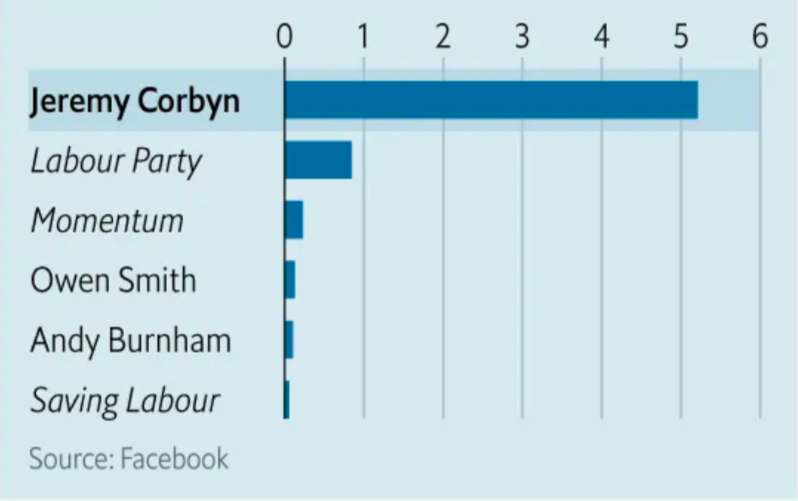
\includegraphics[width=0.6\textwidth]{
    ../graphics/correct-left-click.png
  } 
\end{figure}

\noindent
Replication.

\pgfplotstableread[%
col sep=comma,%
colums/name/.style=string type%
]{%
  ./data/corbyn-data.csv%
}\datatable

\begin{figure}[h]
  \centering

  \begin{tikzpicture}[plotBackground]
    
    \begin{axis}[
      xbar,
      xmin=0,
      xticklabel pos=upper,
      enlarge x limits={value=0.2, upper},
      x coord trafo/.code={\pgfmathparse{\pgfmathresult/1000}},
      xticklabel=\pgfmathprintnumber{\tick},
      x axis line style={draw=none},
      xmajorgrids=true,
      % y axis
      yticklabels from table={\datatable}{name},
      ytick=data,
      y dir=reverse,
      axis y line=left,
      enlarge y limits=0.1,
      y axis line style={-,thick},
      % general
      tick style={draw=none},
      bar width=0.45cm,
      ]
      \addplot[plotBlue, fill=plotBlue]
      table [y expr=\coordindex, x=count] {\datatable};
   \end{axis}
   \node[below left,color=gray] () {\small Source: Facebook};
  \end{tikzpicture}
\end{figure}

\pagebreak
\section{Cherry Picking}
\subsubsection{Source}
\begin{figure}[h]
  \centering
  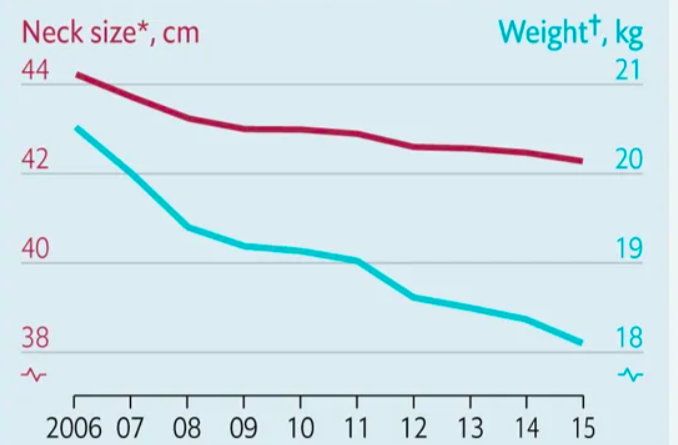
\includegraphics[width=0.7\textwidth]{
    ../graphics/correct-cherry-pick.png
  }
\end{figure}


\subsubsection{Replication}
\pgfplotstableread[%
col sep=comma,%
colums/name/.style=string type,%
colums/year/.style=string type,%
]{%
  ./data/dog-data.csv%
}\datatable

\pgfplotstabletypeset{\datatable}

\begin{figure}[h]
  \centering
  \begin{tikzpicture}[plotBackground]

        
    \begin{axis}[
      scale only axis,
      % plot size
      width=0.7\textwidth,
      height=5cm,
      % x axis
      xtick={0,...,15},
      xticklabels from table={\datatable}{year},
      % xtick=data,
      axis x line=bottom,
      x axis line style={-,thick},
      x tick style={-,thick,black},
      % y axis
      tick align=outside,
      y tick style={draw=none},
      axis y line*=left,
      y axis line style={draw opacity=0},
      yticklabel pos=upper,
      ymajorgrids=true,
      ymax=44.5,
      ymin=38,
      ]  

      \addplot[plotRed, ultra thick]
      table [
      % x expr=\coordindex,
      x expr=\coordindex,
      y=neck,
      ] {\datatable};
    \end{axis}

    \begin{axis}[
      scale only axis,
      % plot size
      width=0.7\textwidth,
      height=5cm,
      % x axis
      axis x line=none,
      % enlarge y limits=0.1,
      % y axis
      axis y line*=right,
      y axis line style={draw opacity=0},
      y tick style={draw=none},
      yticklabel pos=upper,
      ymax=21,
      ymin=17.5,
      ]

      \addplot[plotCyan, ultra thick]
      table [
      % x expr=\coordindex,
      x=year,
      y=weight,
      ] {\datatable};
    \end{axis}
    
  \end{tikzpicture}
\end{figure}


\end{document}